\documentclass[a4paper]{article}

\author{Hidde-Jan Jongsma}
\title{Finite Difference Methods}
\date{\today}

\usepackage{amsmath}
\usepackage{mathtools}

\usepackage{tikz}

\newcommand{\dux}{\frac{\partial u}{\partial x}}
\newcommand{\duxx}{\frac{\partial^2 u}{\partial x^2}}
\newcommand{\duxxx}{\frac{\partial^3 u}{\partial x^3}}

\newcommand{\duy}{\frac{\partial u}{\partial y}}
\newcommand{\duyy}{\frac{\partial^2 u}{\partial y^2}}
\newcommand{\duyyy}{\frac{\partial^3 u}{\partial y^3}}
\newcommand{\lapu}{\nabla^2 u}

\begin{document}

\section{Helmholtz equation}

An important parial differential equation in engineering is the
\emph{Laplace equation}. In two dimensions, it has the following form:
\begin{equation}
  \lapu = \duxx + \duyy = 0.
\end{equation}
When there is a non-zero forcing term, the equation is called the
\emph{Poisson equation}:
\begin{equation}
  \lapu = g(x, y).
\end{equation}
They are both examples of \emph{elliptic} equations. Finite Difference
Methods are often used to solve this kind of problems. We will derive
some of the specific applications of FDM in one and two dimensions.
The Helmholtz problem considers an unknow, but uniquely determined function.
Suppose we have a region $R$ in the $xy$-plane, on which the function
$u = u(x, y)$ takes its values. Here, $u$ satisfies
\begin{equation}
  \begin{dcases*}
    \lapu + f u = g & \\
    u(x, y) = q(x, y) & on boundary of $R$,
  \end{dcases*}
\end{equation}
with $f = f(x, y)$ and $g = g(x, y)$ smooth functions defined on $R$.

\section{FDM 1D Case}

All Finite Difference Methods are created by discritizing $u$ on a grid
on $R$. The second derivative of $u$ at a certain point in $R$  is
approximated by taking a linear combination of the values of $u$ at
the neighbouring points.

\begin{align}
  u_{i + 1} & = u_i + h \dux + \frac{h^2}{2} \duxx + \frac{h^3}{6} \duxxx
                + \frac{h^4}{24} \frac{\partial^4 u}{\partial x^4} + \mathcal{O}(h^5) \\
%
  u_{i - 1} & = u_i - h \dux + \frac{h^2}{2} \duxx - \frac{h^3}{6} \duxxx
                + \frac{h^4}{24} \frac{\partial^4 u}{\partial x^4} + \mathcal{O}(h^5)
\end{align}

By adding these two Tailor series, we obtain an estimate for the second order derivative of
$u$ at $x_i$:
\begin{equation}
  \duxx \approx \frac{1}{h^2}[ u_{i + 1} - 2 u_i + u_{i - 1} ]
          + \frac{h^2}{12} \frac{\partial^4 u}{\partial x^4}.
\end{equation}
We see that this approximation is second order accurate.

\begin{figure}
  \label{fig:1dcase}
  \begin{center}
    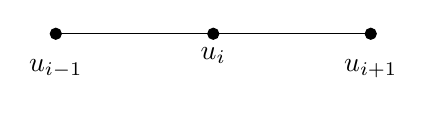
\begin{tikzpicture}

      \tikzstyle{every node}=[draw,circle,fill=black,minimum size=4pt,
                            inner sep=0pt]

      %\tikzstyle{every label}=[distance=5mm]

      \draw (0,0) node (-) [label=below:$u_{i - 1}$] {}
          -- ++(0:2.0cm) node (0) [label=below:$u_{i}$] {}
          -- ++(0:2.0cm) node (+) [label=below:$u_{i + 1}$] {};

    \end{tikzpicture}
  \end{center}
  \caption{Image comes here}
\end{figure}

TODO:
\begin{itemize}
  \item Grid size
  \item 2D case
    \begin{itemize}
      \item Five point stencil
      \item Nine point stencil
    \end{itemize}
\end{itemize}


\end{document}
